%%%%% fs-run-time-model  Computational  Model

\label {fs-model-section}
In our model the dataflow is represented by a directed graph. This graph does not contain information about physical deployment, so further we call it {\it logical} graph or stream. Items are get into the stream through the node called {\it front} and get out through the node called {\it sink}. Fronts and sinks are detailed in the next section; now it is only important that fronts and sinks play the role of the graph enter and graph exit correspondingly. Each other node of the logical graph contains single operation, also called job. Edges show the order of these operations. The data items are processed one-by-one in a "streaming" manner. 

Notably, despite the fact that commonly dataflow graphs assumed to be acyclic (DAGs), our model does not have this restriction. Moreover, as we show further in this section, there are cases when cycles are required, e.g. for reduce step in MapReduce-based algorithms. 

In this section, firstly, the structure of items in the data stream is defined. After that, supported operations and their properties are introduced. Finally, the way to implement any MapReduce transformation using our model is described.

\subsection{The structure of data items}
Generally, the items of the stream are represented as payload and meta-information. It should be highlighted that meta-information is not provided by business logic. Instead of this, it is assigned when the payload element arrives to the front. 

\[DataItem := (payload, Meta)\]

The meta-information of data item is represented as {\it global time} and the trace of {\it local times}.

\[Meta := (GlobalTime, Trace)\]

Global time is assigned to data item once when the item enters the system. It is represented as the concatenation of nanoseconds since the epoch start and the identifier of front. Firstly, such design makes global time strongly monotonic relating to the single front. Secondly, it avoids assigning the same global time for distinct input elements. Global times can be compared lexicographically.

\[GlobalTime := (frontTs, frontId)\]

Local time is the concatenation of logical time of operation and the ordinal number of output item which we call {\it child id}. The logical time is represented as simple items counter within each operation. Therefore, child id is required, because some jobs can generate multiple items from one, e.g. flat map. The items with the same child id are called {\it brothers}. When the item is ready to go out from the operation, its trace of local times is appended by new corresponding local time. The traces of local times can be compared lexicographically.

\[Trace := [LocalTime]\]
\[LocalTime := (logicalTime, childId)\]

Notably, in spite of the fact that initially there are no items with the same global time, they can be generated by some operations. The trace of local times is used to distinguish two elements with the same global time. The main purpose of such approach is to provide information for items invalidation which is detailed in the next section.

The metas can be compared lexicographically: initially by global time and then by the trace of local times.

\subsection{Supported operations}
The set of available operations is limited by the following list.

{\bf Map} applies specified transformation to the payload of input item. Global time of the item is not changed and the trace of local times is appended by the new corresponding element.

{\bf Flat map} applies specified function to the payload of input item. This function returns a sequence of new payloads. Each of these payloads is put into distinct data item. Output items inherit global time from the initial. The traces of output items are appended by local times with the same logical time but distinct child id.

{\bf Filter} applies specified predicate to the payload of input item. If the result of predicate is positive, filter outputs initial item with updated trace of local times. Otherwise, filter outputs nothing.

{\bf Broadcast} replicates input item to the specified number of operations or sinks. Similarly to the flat map, the traces of replicated items are appended by local times with the same logical time but distinct child id. Broadcast is the only operation with multiple outputs.

{\bf Merge} operation is initialized with specified number of input nodes. Each input item from all input nodes is sent to the single output. It should be mentioned that merge operation does not provide any guarantees about the order of items. Global time of the item is not changed and the trace of local times is appended by the new corresponding element. Merge is the only operation with multiple inputs.

{\bf Grouping} has two properties: number called {\it window} and hash function. Grouping stores input items in distinct buckets by the value of the hash function applied to payload. When next in turn item is got in the grouping, it is put to the tail of corresponding bucket. After that, grouping outputs {\it tuple item}, which consists of the last window items of this bucket. If the size of bucket is less than window, all items of bucket are taken. Notably, grouping is the only operation that maintains state.
	
To completely clarify the semantics of this operation, consider the following example. The grouping accepts items with payload represented as natural numbers: 1,2,3, etc. The hash function returns 1 if the number is even and 0 otherwise. If the window is set to 3, the output is:

\[(1), (2), (1|3), (2|4), (1|3|5), (2|4|6), (3|5|7), (4|6|8)...\]

As it can be observed, the result of operation depends on the order of the input items. Currently, we assume that all items are got in the grouping in order defined by global time. The implementation details are described in the next section. 

The important property of the grouping is that the result is uniquely determined by the last element in the tuple. Therefore, grouping is the bijective mapping. Additionally, the results among items with different values of hash function are independent.

Tuple item inherits global time from the last element. The trace of tuple item is the trace of the last item appended with the corresponding local time.  

Figure~\ref{logical-graph-ops-figure} shows the topology of each operation and how it affects the trace of local times.

\begin{figure}[htbp]
  \centering
  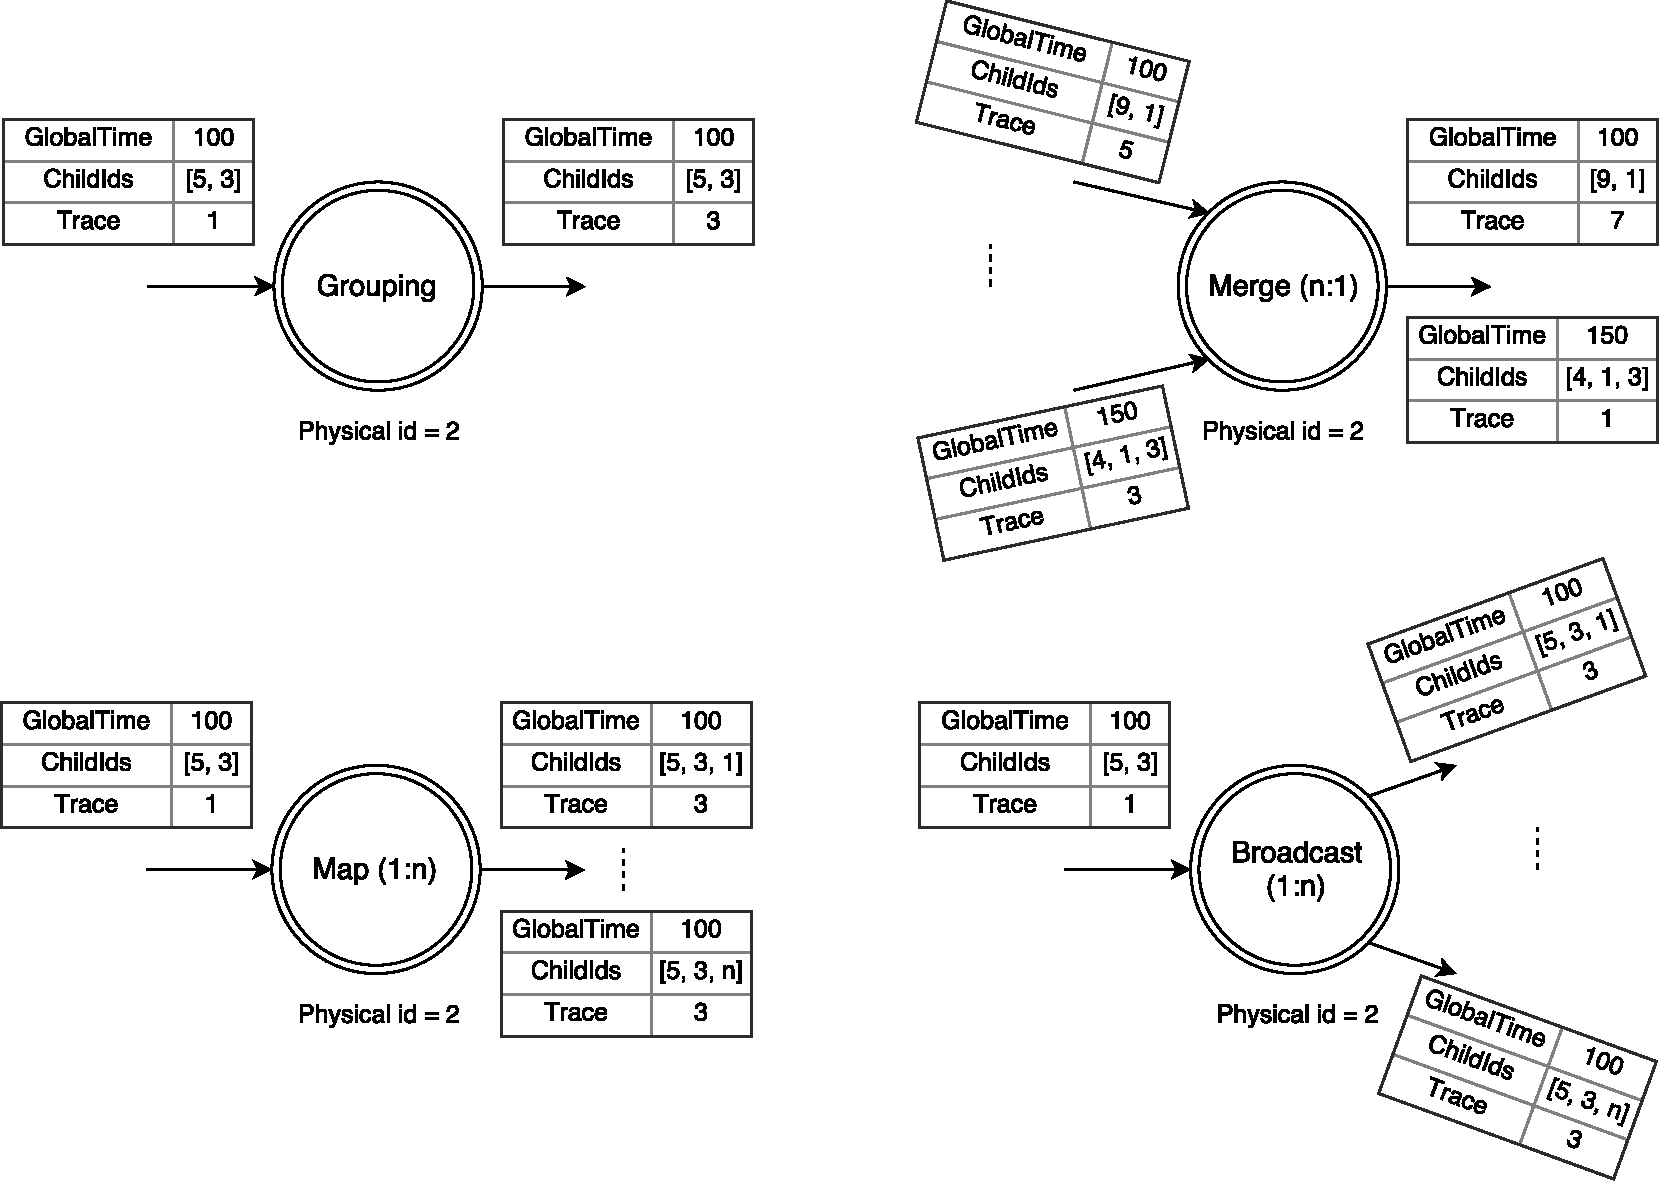
\includegraphics[width=0.48\textwidth]{pics/operations}
  \caption{Supported operations}
  \label {logical-graph-ops-figure}
\end{figure}

\subsection{MapReduce transformations on stream}

\begin{figure}[htbp]
  \centering
  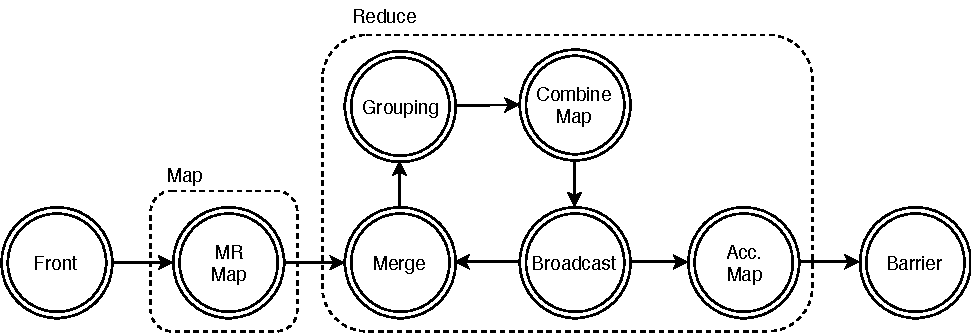
\includegraphics[width=0.48\textwidth]{pics/mapreduce}
  \caption{Logical graph for MapReduce transformations}
  \label {logical-graph-figure}
\end{figure}

Consider the dataflow that is shown on the figure~\ref {logical-graph-figure}. Data items of this stream are: {\it input} items, {\it mapped} items, and {\it reduced} items. Each type of item and the way they were generated are detailed further in this section. However, it is worth to mention that mapped and reduced items have key-value structure of payload. The operations of the stream have the following properties:

\begin{itemize}
\item The first map operation accepts input items and outputs mapped items, according to the business logic. This operation is semantically matched with map step of MapReduce model. Additionally, it should be noted that stream onwards can contain only mapped and reduced items.
\item Merge operation is used for cycle implementation.
\item The window of grouping is set to 2. The hash function is designed to return distinct values for payloads with distinct keys.
\item Filter operation removes tuples with structure \textit{(mapped item; reduced item)}, i.e. tuples, where mapped item was generated before reduced item.
\item The all possible inputs of the second map are the following tuples: \textit{(mapped item), (mapped item; reduced item)}. Any other tuples cannot get in this map because of the filter operation and assumption about the order of items which get in grouping. The first type of input tuples is transformed into reduced item with key inherited from mapped item and some initial value.  The second type is converted into reduce item with the same key. The value of this item is the result of specified reduce function applied to the values of tuple items. Actually, this transformation is equivalent to the reduce step of MapReduce model.
\item Broadcast operation is used for cycle implementation.
\end{itemize}

According to the provided logical graph, any MapReduce transformation can be implemented using the sequence of map, merge, grouping, filter, and broadcast operations. The key idea is that each mapped item is grouped into tuple with corresponding reduced item and then they are combined into the new reduced item. The cycle gives ability for new reduced items to get in grouping operation. Thereby, the stream reacts to each input item by generating new reduced item, which contains the actual value of the reduce step. 

The grouping operation plays the important role in this workflow. Filter operation can remove tuple {\it (mapped item; reduced item)} because of the assumption that grouping accepts items in order relating to the global time. If filter accepts tuple {\it (mapped item; reduced item)}, then it means that mapped item was generated before reduced item, and therefore, it had been already reduced. Moreover, this assumption guarantees that each mapped item would be grouped with the actual reduced item, because grouping always accepts the actual reduced item before new mapped item.

The example of input/output items, which are generated/ transformed by the part of the logical graph, is shown on the figure~\ref {word-count-figure}. This example represents classical MapReduce-based algorithm for word counting. Map step of this algorithm transforms each input word into key-value pair where word is the key, and the value is 1. Reduce step sums all values into the final result for specific key. According to our graph for MapReduce transformations, the item {\it m[dog, 1]/r[dog, 1]} represents mapped/reduced item with key "dog" and value 1. The figure shows how the model reacts on two consequent input items containing word "dog". The meta-information of items is omitted for simplification.

\begin{figure}[htbp]
  \centering
  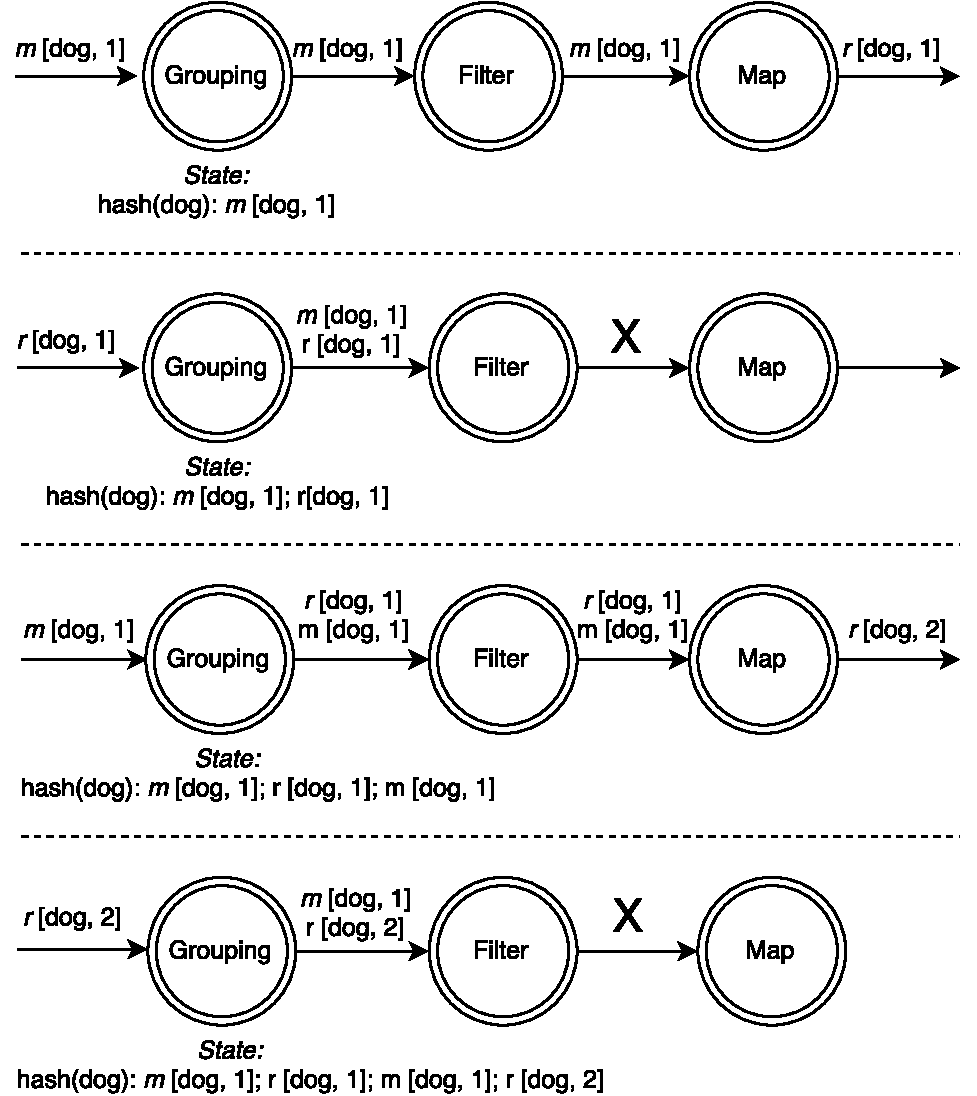
\includegraphics[width=0.48\textwidth]{pics/wordcount}
  \caption{Part of the stream evalutaion for word counting}
  \label {word-count-figure}
\end{figure}

